\chapter{Proposed Approach}
\label{chap:approach}
\section{Introduction}

This chapter describes the fake news detection framework, its datasets and preprocessing steps, and the construction of the BiLSTM, BERT, and hybrid BERT + BiLSTM models.

The proposed detection system is designed as a multi-stage pipeline that converts unstructured news input into a classified output with an associated confidence estimate. Figure~\ref{fig:systemmodel} illustrates the overall system architecture.

\begin{figure}[H]
    \centering
    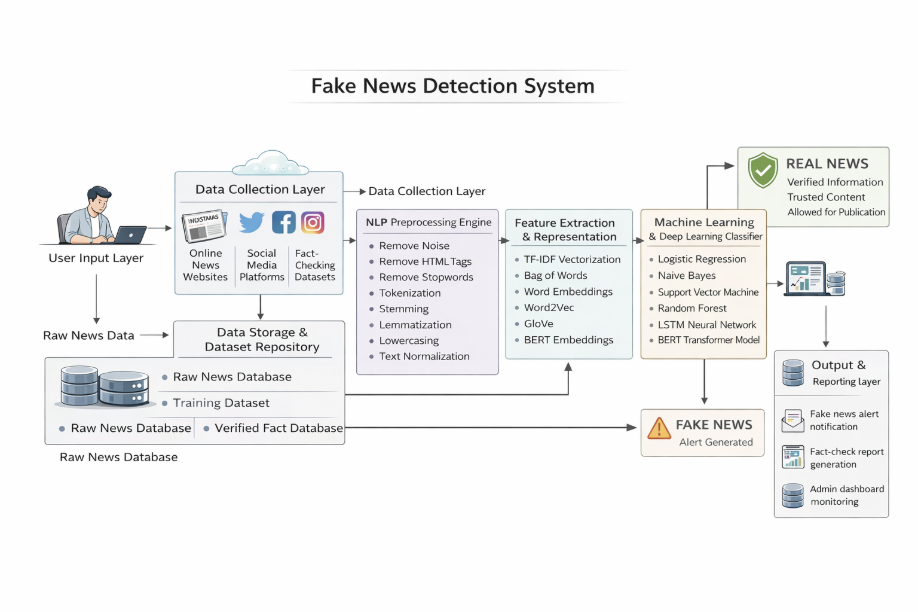
\includegraphics[width=\textwidth,height=0.28\textheight,keepaspectratio]{architecture.png}
    \caption{End-to-end fake news detection system pipeline, from user input through data collection, NLP preprocessing, feature extraction, classification, and output reporting}
    \label{fig:systemmodel}
\end{figure}

The pipeline is organized into the following stages:

\begin{itemize}
\item \textbf{User Input Layer:} Accepts raw news input in the form of free text, a headline, or a URL pointing to a news article.
\item \textbf{Data Collection Layer:} Gathers the corresponding data from benchmark datasets (LIAR, ISOT, FakeNewsNet) and, where applicable, online news websites, social media platforms, and fact-checking sources.
\item \textbf{Data Storage and Dataset Repository:} Persists raw news data, training/validation/test splits, and verified fact databases for reuse across experiments.
\item \textbf{NLP Preprocessing Engine:} Cleans and normalizes the raw text through noise removal, HTML-tag stripping, stopword removal, tokenization, stemming, lemmatization, and lowercasing, as described in Section~\ref{sec:preprocessing}.
\item \textbf{Feature Extraction and Representation Layer:} Converts the normalized text into numeric representations using TF-IDF, Bag-of-Words, Word2Vec, GloVe, and/or BERT embeddings, depending on the downstream classifier.
\item \textbf{Machine Learning and Deep Learning Classifier:} Hosts the candidate classification models compared in this thesis -- BiLSTM, BERT, and the hybrid BERT + BiLSTM model -- and produces a REAL/FAKE prediction with a confidence score.
\item \textbf{Output and Reporting Layer:} Emits the final classification decision together with a human-readable report, suitable for downstream use cases such as a fake-news alert notification, a fact-check report, or an administrative monitoring dashboard.
\end{itemize}

This layered design cleanly separates preprocessing, representation, and modelling concerns, which makes it straightforward to swap in the three candidate classifiers (BiLSTM, BERT, BERT + BiLSTM) without changing the surrounding pipeline.

\section{Dataset Description}

All experimental evaluations are performed using benchmark datasets widely used in the fake news detection literature: LIAR~\citep{Wang2017Liar}, ISOT~\citep{ISOTDataset}, and FakeNewsNet~\citep{Shu2020FakeNewsNet}. Table~\ref{tab:datasets} summarizes the size and composition of each dataset. A Kaggle-hosted version of these benchmark datasets was used for training and evaluation.

\begin{table}[htbp]
\small
\setlength{\tabcolsep}{3pt}
\centering
\caption{Dataset Description}
\label{tab:datasets}
\begin{tabularx}{\textwidth}{|l|r|r|r|X|}
\hline
\textbf{Dataset} & \textbf{Total Samples} & \textbf{Real News} & \textbf{Fake News} & \textbf{Source} \\ \hline
LIAR & 12,836 & 6,418 & 6,418 & PolitiFact Statements \\
ISOT & 44,919 & 21,417 & 23,502 & Reuters \& Fake News Sites \\
FakeNewsNet & 23,196 & 11,941 & 11,255 & PolitiFact \& GossipCop \\ \hline
\end{tabularx}
\end{table}

Each dataset was split in an 80:10:10 ratio, corresponding to the training, validation, and testing sets respectively, in accordance with established conventions in the literature~\citep{Kaliyar2021FakeBERT,Rai2022FakeNews}.

\section{Data Preprocessing}
\label{sec:preprocessing}

Raw news text is noisy: it contains inconsistent casing, punctuation, HTML artifacts, and words that carry little discriminative signal. Before any feature extraction or model training can take place, the text must be cleaned and normalized. The standard NLP preprocessing pipeline used in this thesis consists of the following steps:

\begin{itemize}
\item \textbf{Noise Removal:} Stripping HTML tags, special characters, URLs, and other non-textual artifacts from the raw input.
\item \textbf{Lowercasing:} Converting all text to a consistent case so that, e.g., ``News'' and ``news'' are treated identically.
\item \textbf{Tokenization:} Splitting text into individual tokens (words or sub-word units), which form the atomic units consumed by downstream models.
\item \textbf{Stopword Removal:} Removing high-frequency, low-information words (e.g., ``the'', ``is'', ``and'') that do not contribute to distinguishing fake from real news.
\item \textbf{Stemming and Lemmatization:} Reducing words to their root or base form (e.g., ``running'' $\rightarrow$ ``run''), which reduces vocabulary size and helps models generalize across word forms.
\item \textbf{Padding / Truncation:} Normalizing the length of tokenized sequences to a fixed maximum length so that they can be processed in fixed-size batches by neural network models.
\end{itemize}

For transformer models such as BERT, tokenization is performed using a model-specific sub-word tokenizer (WordPiece), and two special tokens are introduced: a classification token, \texttt{[CLS]}, prepended to every sequence and used to aggregate sequence-level information, and a separator token, \texttt{[SEP]}, used to mark sequence boundaries. Each tokenized sequence is accompanied by an attention mask that indicates which positions correspond to real tokens (1) versus padding (0), so that the model does not attend to padded positions.

\section{Model Building}

All three models were trained using hyperparameters appropriate to their architecture, so that the comparison remains fair while respecting each model family's characteristics. BERT-based models use a lower learning rate and smaller batch size than BiLSTM, since they are already pre-trained and only require fine-tuning, whereas the standalone BiLSTM model, trained from scratch, uses a higher learning rate. Table~\ref{tab:hyperparameters} lists the exact configuration used for each model.

\begin{table}[htbp]
\setlength{\tabcolsep}{3pt}
\centering
\caption{Hyperparameter Configuration of Models}
\label{tab:hyperparameters}
\small
\begin{tabularx}{\textwidth}{|>{\raggedright\arraybackslash}X|>{\centering\arraybackslash}X|>{\centering\arraybackslash}X|>{\centering\arraybackslash}X|}
\hline
\textbf{Hyperparameter} & \textbf{BiLSTM} & \textbf{BERT} & \textbf{BERT + BiLSTM} \\ \hline
Embedding Type & GloVe & BERT Base & BERT Base \\ \hline
Max Sequence Length & 200 & 256 & 256 \\ \hline
Hidden Units & 128 & --- & 128 \\ \hline
Number of Layers & 2 & 12 (Transformer) & 12 + BiLSTM \\ \hline
Dropout Rate & 0.5 & 0.1 & 0.3 \\ \hline
Batch Size & 32 & 16 & 16 \\ \hline
Learning Rate & 0.001 & 2e-5 & 2e-5 \\ \hline
Optimizer & Adam & AdamW & AdamW \\ \hline
Epochs & 3 & 3 & 3 \\ \hline
Loss Function & Binary Crossentropy & Crossentropy & Crossentropy \\ \hline
\end{tabularx}
\end{table}

\subsection{Fake News Detection Using BiLSTM}

Long Short-Term Memory (LSTM) networks are a class of Recurrent Neural Networks (RNNs) specifically designed to model sequential data while mitigating the vanishing gradient problem that plagues vanilla RNNs over long sequences. An LSTM cell maintains an internal memory state that is selectively updated, forgotten, and output at each time step through a set of learned gates (input, forget, and output gates), allowing the network to retain relevant information over longer spans of text than a standard RNN.

A standard LSTM processes a sequence in a single direction, typically left to right, meaning that at any given position, the model has only seen the preceding context. A Bidirectional LSTM (BiLSTM) addresses this limitation by running two LSTM layers over the input sequence in parallel, one processing it left-to-right and the other right-to-left, and concatenating (or otherwise combining) their hidden states at each position. This gives the BiLSTM access to both past and future context, which is particularly useful for understanding a word's role in a sentence.

Despite this improvement, BiLSTM networks still process text strictly sequentially at inference time, which limits parallelization during training, and their capacity to model very long-range dependencies remains weaker than attention-based architectures. Furthermore, BiLSTM models trained with a limited number of epochs and without extensive hyperparameter tuning can converge poorly, resulting in substantially lower accuracy than transformer-based alternatives.

\subsection{Fake News Detection Using BERT}

The Transformer architecture dispenses with recurrence entirely and instead relies on a self-attention mechanism, which allows every token in a sequence to directly attend to every other token in a single layer, regardless of their distance in the sequence. This removes the sequential bottleneck of RNN-based models and enables far greater parallelization during training, while also making it easier to model long-range dependencies.

BERT (Bidirectional Encoder Representations from Transformers) is built from a stack of Transformer encoder layers (12 layers in the BERT-Base configuration) and is pre-trained on large unlabelled text corpora using two self-supervised objectives: masked language modelling (predicting randomly masked tokens from their context) and next sentence prediction. This pre-training allows BERT to learn deep, bidirectional, general-purpose language representations before it is ever exposed to a downstream task.

For a downstream classification task such as fake news detection, a pre-trained BERT model is \textit{fine-tuned}: the input news text is tokenized and fed through the pre-trained encoder, producing a contextual embedding for every token, including the special \texttt{[CLS]} token, which is conventionally used as an aggregate representation of the entire sequence. A lightweight classification head (typically a dropout layer followed by a fully connected layer with a softmax or sigmoid activation) is then trained on top of this representation to predict the real/fake label, while the underlying BERT weights are also updated (fine-tuned) using a comparatively small learning rate, since they are already well-initialized from pre-training.

In the hybrid architecture examined in this thesis (Section~\ref{sec:hybrid}), rather than relying solely on the \texttt{[CLS]} token, the entire sequence of contextual token embeddings produced by BERT is passed into a BiLSTM layer, allowing the network to additionally model sequential dependencies over BERT's already contextualized representations before final classification.

\subsection{Fake News Detection Using BERT + BiLSTM}
\label{sec:hybrid}

While the system model in Figure~\ref{fig:systemmodel} shows the pipeline at a high level, Figure~\ref{fig:architecture} zooms into the detailed architecture of the hybrid BERT + BiLSTM model.

\begin{figure}[H]
    \centering
    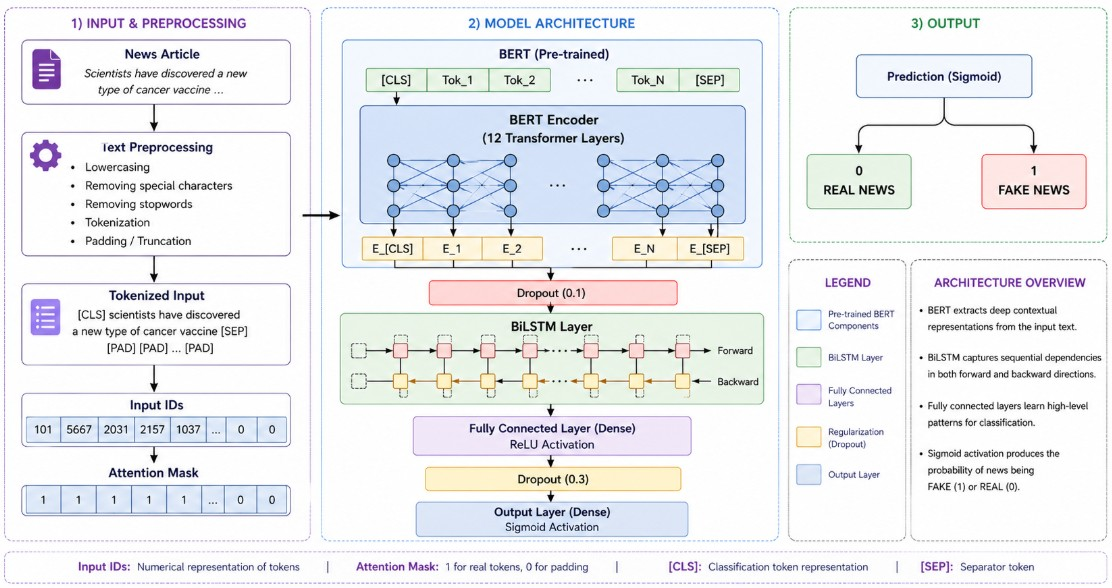
\includegraphics[width=\textwidth,height=0.65\textheight,keepaspectratio]{Arch.jpg}
    \caption{Detailed architecture of the proposed BERT + BiLSTM fake news detection model}
    \label{fig:architecture}
\end{figure}

As shown in the figure, the input news article is first tokenized and normalized (lowercasing, special-character removal, stopword removal, tokenization, padding/truncation), producing a fixed-length sequence of token IDs together with an attention mask. This tokenized sequence, prefixed with a \texttt{[CLS]} token and suffixed with a \texttt{[SEP]} token, is passed through a pre-trained BERT encoder consisting of 12 Transformer layers, which produces a contextual embedding for every token position ($E_{[CLS]}, E_1, \ldots, E_N, E_{[SEP]}$).

Rather than discarding all but the \texttt{[CLS]} embedding, as is common in simple BERT fine-tuning setups, the proposed model passes the entire sequence of contextual embeddings through a dropout layer (rate 0.1) and then into a BiLSTM layer, which processes the sequence in both forward and backward directions to capture sequential dependencies over BERT's already-contextualized representations. The output of the BiLSTM layer is passed through a fully connected (dense) layer with a ReLU activation, followed by a second dropout layer (rate 0.3), and finally an output dense layer with a sigmoid activation that produces the probability of the input being fake (1) or real (0).

the two model families have complementary strengths that motivate the hybrid design explored here. BERT excels at capturing context and semantics within text through its bidirectional Transformer design and self-attention mechanism, but its primary mechanism for aggregating sequence-level information is attention rather than explicit sequence modelling of the kind performed by recurrent networks.

BiLSTM, on the other hand, is purpose-built for modelling sequences and capturing temporal/positional dependencies in text, processing its input in both forward and backward directions. In the proposed hybrid framework, BERT acts as a contextual feature extractor that produces informative token-level embeddings; rather than depending solely on the \texttt{[CLS]} token, the entire sequence of contextual embeddings generated by BERT is fed into the BiLSTM layer, allowing the network to layer explicit sequential modelling on top of BERT's already rich contextual representations.

Consequently, the resulting BERT + BiLSTM framework is designed to benefit from both contextual embeddings (BERT) and sequential learning (BiLSTM). The comparison uses the training configuration reported in Table~\ref{tab:hyperparameters}.

% Original chapter retained below, including excluded problem statement, algorithm, and summary.
% \sloppy
% \chapter{Proposed Approach}
% \addtocontents{toc}{\protect\setcounter{tocdepth}{2}}
% \section{Introduction}
% 
% This chapter describes the fake news detection system proposed and evaluated in this thesis. It begins with a formal problem statement, then presents the overall system model as an end-to-end pipeline, followed by a detailed description of the proposed BERT + BiLSTM classification architecture, the underlying algorithm, and the design rationale for combining a transformer encoder with a sequential BiLSTM layer.
% 
% \section{Problem Statement}
% 
% Given a piece of news text $T$ (an article body, headline, or short statement), the goal is to learn a classification function $f(T) \rightarrow \{\text{REAL}, \text{FAKE}\}$ that predicts whether $T$ represents genuine or fabricated/misleading news, along with an associated confidence score. The function $f$ must be learned from labelled training data drawn from one or more benchmark datasets, and must generalize not only to unseen examples from the same dataset, but ideally also across datasets with different sources, writing styles, and label distributions (evaluated in this thesis using LIAR and ISOT, as discussed in Chapter~5).
% 
% This thesis specifically investigates three candidate realizations of $f$: a purely sequential deep learning model (BiLSTM), a purely transformer-based model (BERT), and a hybrid model that composes both (BERT + BiLSTM), with the aim of empirically determining which realization offers the best trade-off between detection accuracy, generalization across datasets, and model complexity.
% 
% \section{System Model}
% 
% The proposed detection system is designed as a multi-stage pipeline that converts unstructured news input into a classified output with an associated confidence estimate. Figure~\ref{fig:systemmodel} illustrates the overall system architecture.
% 
% \begin{figure}[H]
%     \centering
%     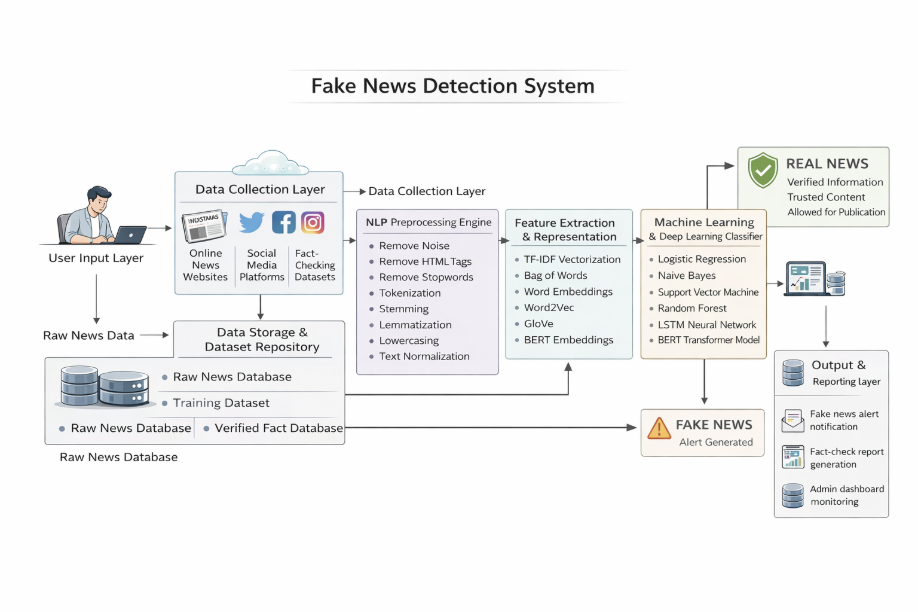
\includegraphics[width=0.95\textwidth]{architecture.png}
%     \caption{End-to-end fake news detection system pipeline, from user input through data collection, NLP preprocessing, feature extraction, classification, and output reporting}
%     \label{fig:systemmodel}
% \end{figure}
% 
% The pipeline is organized into the following stages:
% 
% \begin{itemize}
% \item \textbf{User Input Layer:} Accepts raw news input in the form of free text, a headline, or a URL pointing to a news article.
% \item \textbf{Data Collection Layer:} Gathers the corresponding data from benchmark datasets (LIAR, ISOT, FakeNewsNet) and, where applicable, online news websites, social media platforms, and fact-checking sources.
% \item \textbf{Data Storage and Dataset Repository:} Persists raw news data, training/validation/test splits, and verified fact databases for reuse across experiments.
% \item \textbf{NLP Preprocessing Engine:} Cleans and normalizes the raw text through noise removal, HTML-tag stripping, stopword removal, tokenization, stemming, lemmatization, and lowercasing, as detailed in Chapter~2.
% \item \textbf{Feature Extraction and Representation Layer:} Converts the normalized text into numeric representations using TF-IDF, Bag-of-Words, Word2Vec, GloVe, and/or BERT embeddings, depending on the downstream classifier.
% \item \textbf{Machine Learning and Deep Learning Classifier:} Hosts the candidate classification models compared in this thesis -- BiLSTM, BERT, and the hybrid BERT + BiLSTM model -- and produces a REAL/FAKE prediction with a confidence score.
% \item \textbf{Output and Reporting Layer:} Emits the final classification decision together with a human-readable report, suitable for downstream use cases such as a fake-news alert notification, a fact-check report, or an administrative monitoring dashboard.
% \end{itemize}
% 
% This layered design cleanly separates preprocessing, representation, and modelling concerns, which makes it straightforward to swap in the different classifiers evaluated in Chapter~5 (BiLSTM, BERT, BERT + BiLSTM) without changing the surrounding pipeline.
% 
% \section{Proposed BERT + BiLSTM Detection Framework}
% 
% While the system model in Figure~\ref{fig:systemmodel} shows the pipeline at a high level, Figure~\ref{fig:architecture} zooms into the detailed architecture of the best-performing classifier evaluated in this thesis: the hybrid BERT + BiLSTM model.
% 
% \begin{figure}[H]
%     \centering
%     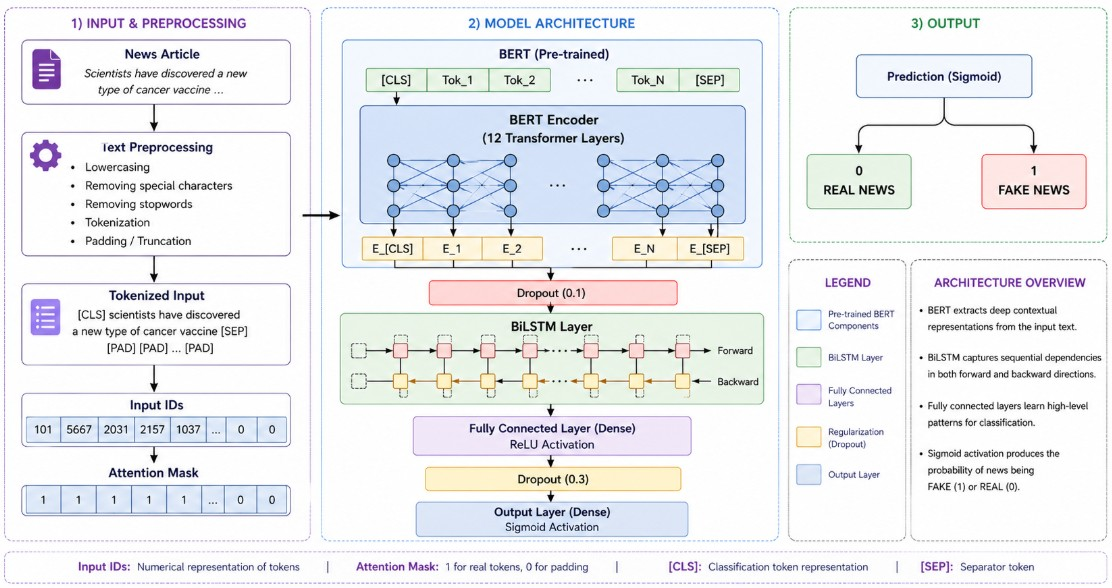
\includegraphics[scale=0.6]{Arch.jpg}
%     \caption{Detailed architecture of the proposed BERT + BiLSTM fake news detection model}
%     \label{fig:architecture}
% \end{figure}
% 
% As shown in the figure, the input news article is first tokenized and normalized (lowercasing, special-character removal, stopword removal, tokenization, padding/truncation), producing a fixed-length sequence of token IDs together with an attention mask. This tokenized sequence, prefixed with a \texttt{[CLS]} token and suffixed with a \texttt{[SEP]} token, is passed through a pre-trained BERT encoder consisting of 12 Transformer layers, which produces a contextual embedding for every token position ($E_{[CLS]}, E_1, \ldots, E_N, E_{[SEP]}$).
% 
% Rather than discarding all but the \texttt{[CLS]} embedding, as is common in simple BERT fine-tuning setups, the proposed model passes the entire sequence of contextual embeddings through a dropout layer (rate 0.1) and then into a BiLSTM layer, which processes the sequence in both forward and backward directions to capture sequential dependencies over BERT's already-contextualized representations. The output of the BiLSTM layer is passed through a fully connected (dense) layer with a ReLU activation, followed by a second dropout layer (rate 0.3), and finally an output dense layer with a sigmoid activation that produces the probability of the input being fake (1) or real (0).
% 
% \subsection{Proposed Algorithm}
% 
% The complete classification procedure for the proposed BERT + BiLSTM model is summarized in Algorithm~\ref{alg:bertbilstm}.
% 
% \begin{algorithm}[H]
% \SetAlgoLined
% \KwIn{Raw news text $T$}
% \KwOut{Classification label $y \in \{\text{REAL}, \text{FAKE}\}$ with confidence score}
% Preprocess $T$: apply noise removal, lowercasing, tokenization, stopword removal, and lemmatization\;
% Tokenize the preprocessed text using BERT's WordPiece tokenizer, prepend \texttt{[CLS]} and append \texttt{[SEP]}\;
% Pass the tokenized sequence through the pre-trained BERT encoder to obtain contextual embeddings $E_{[CLS]}, E_1, \ldots, E_N, E_{[SEP]}$\;
% Apply dropout to the sequence of contextual embeddings\;
% Pass the embedding sequence through a BiLSTM layer to obtain sequence-aware hidden representations\;
% Pass the BiLSTM output through a fully connected layer with ReLU activation\;
% Apply dropout, then pass the result through an output dense layer with sigmoid activation\;
% \Return{predicted label $y$ (REAL or FAKE) and its associated confidence score}\;
% \caption{Fake News Detection using the Proposed BERT + BiLSTM Model}
% \label{alg:bertbilstm}
% \end{algorithm}
% 
% \subsection{Design Rationale: Why Combine BERT and BiLSTM?}
% 
% It is worth emphasizing that the motivation for combining BERT and BiLSTM is not that BiLSTM performs poorly on its own (although, as shown in Chapter~5, it does under the training conditions used in this thesis). Rather, the two model families have complementary strengths that motivate the hybrid design explored here. BERT excels at capturing context and semantics within text through its bidirectional Transformer design and self-attention mechanism, but its primary mechanism for aggregating sequence-level information is attention rather than explicit sequence modelling of the kind performed by recurrent networks.
% 
% BiLSTM, on the other hand, is purpose-built for modelling sequences and capturing temporal/positional dependencies in text, processing its input in both forward and backward directions. In the proposed hybrid framework, BERT acts as a contextual feature extractor that produces informative token-level embeddings; rather than depending solely on the \texttt{[CLS]} token, the entire sequence of contextual embeddings generated by BERT is fed into the BiLSTM layer, allowing the network to layer explicit sequential modelling on top of BERT's already rich contextual representations.
% 
% Consequently, the resulting BERT + BiLSTM framework is designed to benefit from both contextual embeddings (BERT) and sequential learning (BiLSTM). Whether this theoretical complementarity translates into a measurable accuracy improvement in practice -- and under what training conditions it might -- is examined empirically in Chapter~5.
% 
% \section{Summary}
% 
% This chapter has presented the proposed fake news detection system: a formal problem statement, an end-to-end system pipeline spanning input collection through NLP preprocessing, feature extraction, classification, and reporting, and a detailed description of the proposed BERT + BiLSTM classification architecture, its algorithm, and the design rationale behind combining a transformer encoder with a sequential BiLSTM layer. Chapter~5 evaluates this proposed model, together with the standalone BiLSTM and BERT baselines, on multiple benchmark datasets.
% 
